\documentclass[a4paper,10pt]{article}
\usepackage[margin=14mm,top=12mm,bottom=13mm]{geometry}
\usepackage[T1]{fontenc}
\usepackage{helvet}
\renewcommand{\familydefault}{\sfdefault}
\usepackage{microtype}
\usepackage{array,booktabs,tabularx,longtable,amssymb,colortbl}
\usepackage{xcolor}
\usepackage{tikz}
\usetikzlibrary{arrows.meta,positioning}
\usepackage[most]{tcolorbox}
\usepackage{enumitem}
\usepackage{hyperref}
\usepackage{xurl}
\pagestyle{empty}
\setlength{\parindent}{0pt}
\setlength{\parskip}{2.5pt}
\setlist[itemize]{leftmargin=4mm,itemsep=1.0pt,topsep=1.5pt,parsep=0pt}
\setlist[enumerate]{leftmargin=5mm,itemsep=1.0pt,topsep=1.5pt,parsep=0pt}

\definecolor{VMTeal}{HTML}{006C78}
\definecolor{VMDark}{HTML}{143C50}
\definecolor{VMLight}{HTML}{EAF5F5}
\definecolor{VMGold}{HTML}{C98314}
\definecolor{VMGreen}{HTML}{1F8A55}
\definecolor{VMGray}{HTML}{F3F5F6}
\definecolor{VMRed}{HTML}{A33B36}
\hypersetup{colorlinks=true,urlcolor=VMTeal,linkcolor=VMTeal}

\newtcolorbox{vmBox}[2][]{
  enhanced,
  colback=white,
  colframe=VMTeal,
  boxrule=0.55pt,
  arc=1.5mm,
  left=2.2mm,right=2.2mm,top=2.2mm,bottom=1.9mm,
  title={#2},
  coltitle=VMDark,
  fonttitle=\bfseries\fontsize{10.2}{11.2}\selectfont,
  attach boxed title to top left={xshift=1.8mm,yshift=-2.0mm},
  boxed title style={colback=white,colframe=white,boxrule=0pt,left=0.5mm,right=0.5mm},
  before skip=1mm,after skip=1mm,
  #1
}

\newtcolorbox{vmHighlight}[1][]{
  enhanced,
  colback=VMLight,
  colframe=VMTeal,
  boxrule=0.5pt,
  arc=1.5mm,
  left=2.5mm,right=2.5mm,top=2mm,bottom=2mm,
  before skip=1mm,after skip=1mm,
  #1
}

\newcommand{\yes}{\textcolor{VMGreen}{\bfseries\checkmark}}
\newcommand{\partmark}{\textcolor{VMGold}{\bfseries$\triangle$}}
\newcommand{\no}{\textcolor{VMRed}{\bfseries--}}
\newcommand{\source}[2]{\textsuperscript{\href{#1}{[#2]}}}
\newcommand{\sectiontitle}[1]{\vspace{1mm}{\fontsize{13}{14}\selectfont\bfseries\color{VMDark}#1}\par\vspace{1mm}}

\begin{document}
\fontsize{8.8}{10.5}\selectfont

% ==================== PAGE 1 ====================
\begin{minipage}[t]{0.73\textwidth}
{\fontsize{21}{22}\selectfont\bfseries\color{VMDark}VentureMath}\par
{\fontsize{11.5}{13}\selectfont\bfseries\color{VMTeal}Uncertainty-Certified AI Compiler for Minimum-Viable Hardware Digital Twins}
\end{minipage}
\hfill
\begin{minipage}[t]{0.24\textwidth}
\raggedleft
\colorbox{VMLight}{\parbox{0.94\linewidth}{\centering\bfseries\color{VMDark}Concept Brief\\[-1pt]\normalfont\fontsize{7.8}{8.8}\selectfont Working draft for internal discussion and collaborator outreach}}
\end{minipage}

\vspace{2mm}

\begin{vmHighlight}
\textbf{Concept in one sentence.} VentureMath converts an early hardware venture idea, manufacturer datasheets, and a minimal set of physical measurements into a traceable, calibrated, and decision-ready simulation before a team commits to a full hardware build.
\end{vmHighlight}

\begin{minipage}[t]{0.49\textwidth}
\begin{vmBox}{Problem and Beachhead Opportunity}
\textbf{Problem.} Generative AI has reduced the expertise required to produce early software prototypes, but hardware venture creation still depends on scarce knowledge in datasheets, embedded systems, mathematical modeling, calibration, and physical testing. Design errors are often discovered only after components are purchased and assembled.

\textbf{Beachhead customers.} University entrepreneurship centers, engineering entrepreneurship programs, capstone courses, campus makerspaces, and university-affiliated incubators supporting student and first-time hardware founders.

\textbf{Gap in current alternatives.}
\begin{itemize}
\item General-purpose LLMs generate plausible but unverified advice.
\item Fixed kits constrain teams to predefined projects.
\item Professional simulators assume expert-built and expert-calibrated models.
\end{itemize}
\end{vmBox}
\end{minipage}
\hfill
\begin{minipage}[t]{0.49\textwidth}
\begin{vmBox}{Core High-Risk Hypothesis}
\textbf{Hypothesis.} Provenance-constrained model synthesis plus active calibration can produce decision-useful digital twins with substantially less expert correction and fewer physical experiments than unconstrained LLM generation or static template-based modeling.

\textbf{High-risk unknown.} Can incomplete venture requirements and heterogeneous datasheets be compiled into cross-component models that are:
\begin{itemize}
\item executable and dimensionally consistent;
\item physically predictive under real non-idealities;
\item uncertainty-calibrated; and
\item able to refuse unsupported predictions?
\end{itemize}
\end{vmBox}
\end{minipage}

\sectiontitle{Proposed Technical Architecture}

\begin{vmBox}{}
\centering
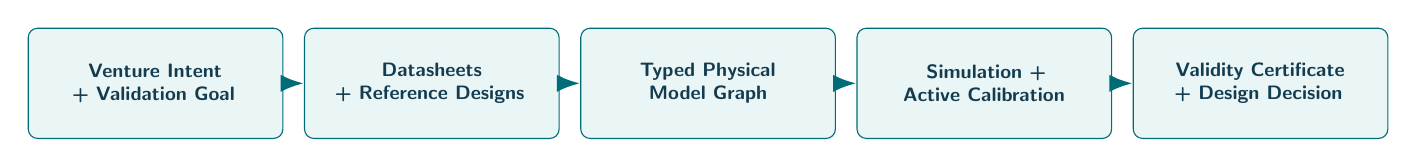
\begin{tikzpicture}[
 node distance=2.6mm,
 box/.style={draw=VMTeal,rounded corners=1.2mm,fill=VMLight,align=center,minimum height=14mm,text width=30mm,font=\fontsize{7.4}{8.3}\selectfont\bfseries,text=VMDark},
 arrow/.style={-Latex,very thick,color=VMTeal}
]
\node[box] (a) {Venture Intent\\+ Validation Goal};
\node[box,right=of a] (b) {Datasheets\\+ Reference Designs};
\node[box,right=of b] (c) {Typed Physical\\Model Graph};
\node[box,right=of c] (d) {Simulation +\\Active Calibration};
\node[box,right=of d] (e) {Validity Certificate\\+ Design Decision};
\draw[arrow] (a)--(b); \draw[arrow] (b)--(c); \draw[arrow] (c)--(d); \draw[arrow] (d)--(e);
\end{tikzpicture}

\vspace{2mm}
\begin{minipage}{0.96\linewidth}
\begin{itemize}
\item \textbf{Grounded compilation:} extract requirements, units, operating ranges, interfaces, validity conditions, calibration relationships, and source provenance.
\item \textbf{Constrained synthesis:} select and instantiate validated primitives for sensing, sampling, noise, communication, power, and low-voltage actuation instead of freely inventing equations.
\item \textbf{Hybrid modeling:} combine first-principles models with compact residual models for bias, noise, delay, and component variation not captured by datasheets.
\item \textbf{Active calibration:} recommend the smallest safe sequence of physical tests expected to reduce uncertainty and distinguish among confounded error sources.
\item \textbf{Validity certification:} report calibrated intervals, supported operating regions, unresolved assumptions, and explicit out-of-domain refusal conditions.
\end{itemize}
\end{minipage}

\vspace{1mm}
\colorbox{VMLight}{\parbox{0.94\linewidth}{\centering\textbf{Phase I technical wedge:} ESP32-S3 connected sensing, Wi-Fi, a curated sensor library, and simple low-voltage actuation.}}
\end{vmBox}

\begin{minipage}[t]{0.49\textwidth}
\begin{vmBox}{Phase I Objectives}
\begin{enumerate}
\item \textbf{Provenance-linked model compiler.} Convert venture intent and component evidence into typed executable model graphs.
\item \textbf{Hybrid modeling and active calibration.} Learn sparse residuals and select informative physical tests.
\item \textbf{Sim-to-real validity certification.} Quantify predictive error, supported regions, and uncertainty coverage.
\end{enumerate}
\end{vmBox}
\end{minipage}
\hfill
\begin{minipage}[t]{0.49\textwidth}
\begin{vmBox}{Measures of Technical Success}
\begin{itemize}
\item Executable-model rate and expert correction time
\item Parameter extraction and provenance completeness
\item Physical prediction error and uncertainty coverage
\item Calibration tests required per model
\item Fault localization accuracy and time to a decision-ready design
\end{itemize}
\end{vmBox}
\end{minipage}

\begin{vmBox}{Team, Preliminary Work, and Collaboration Ask}
\textbf{PI.} Leads mathematical representation, simulation, uncertainty quantification, active experiment design, benchmarking, and overall R\&D execution.

\textbf{Altitut preliminary work.} Provides an existing AI-assisted venture workflow, language-model and datasheet-processing capabilities, platform integration, and relationships with university entrepreneurship programs.

\textbf{Collaboration ask.} Seeking an embedded systems/robotics consultant, university pilot partners, and collaborators in model-based design, digital twins, and engineering education. A prospective EE/robotics advisor has been identified; formal participation remains subject to employer approval or replacement by an equivalent consultant.
\end{vmBox}

\newpage

% ==================== PAGE 2 ====================
{\fontsize{19}{20}\selectfont\bfseries\color{VMDark}VentureMath Prior-Art Matrix}\par
{\fontsize{9.5}{11}\selectfont\color{black!70}Working differentiation relative to adjacent research. Novelty must still be confirmed through a fuller literature, patent, and commercial-product review.}

\vspace{2mm}

\renewcommand{\arraystretch}{1.18}
\setlength{\tabcolsep}{3.0pt}
\fontsize{7.2}{8.5}\selectfont
\begin{tabularx}{\textwidth}{>{\raggedright\arraybackslash}p{24mm} >{\raggedright\arraybackslash}p{48mm} >{\centering\arraybackslash}p{12mm} >{\centering\arraybackslash}p{15mm} >{\centering\arraybackslash}p{17mm} >{\raggedright\arraybackslash}X}
\toprule
\rowcolor{VMDark}
\color{white}\textbf{Approach} & \color{white}\textbf{Primary contribution} & \color{white}\textbf{Venture intent} & \color{white}\textbf{Datasheet grounding} & \color{white}\textbf{Active calibration / UQ} & \color{white}\textbf{Boundary relative to VentureMath} \\
\midrule
\textbf{ModiGen}\source{https://arxiv.org/abs/2503.18460}{1} & Modelica component and test-case generation using fine-tuning, graph RAG, and feedback optimization. & \no & \no & \no & Improves simulation-code generation, but does not begin with venture requirements or establish predictive validity against physical measurements. \\
\rowcolor{VMGray}
\textbf{SimuAgent}\source{https://openreview.net/forum?id=mMB3Y1ERqi}{2} & Agentic Simulink model construction and analysis through compact representation, planning, execution, and reflection. & \partmark & \no & \no & Automates model-building inside an existing environment; does not ground models in manufacturer evidence or certify sim-to-real validity. \\
\textbf{D2S-FLOW}\source{https://arxiv.org/abs/2502.16540}{3} & Extracts electrical parameters from datasheets to generate SPICE device models. & \no & \yes & \no & Strong component-level precedent, but does not compose heterogeneous systems, plan minimal physical tests, or issue a system-level validity certificate. \\
\rowcolor{VMGray}
\textbf{Uncertainty-aware digital twins}\source{https://arxiv.org/abs/2501.10337}{4}\source{https://arxiv.org/abs/2507.01047}{5} & Quantifies uncertainty, performs robust control, active learning, or online updating for an already defined twin or surrogate. & \no & \no & \yes & Addresses uncertainty after a twin is specified; usually assumes an expert-selected scope, variables, equations, and data pipeline. \\
\textbf{VentureMath (proposed)} & Compiles venture goals and component evidence into a typed minimum-viable twin, then performs sparse calibration and explicit predictive-validity certification. & \yes & \yes & \yes & Intended differentiator: jointly address model creation, evidence grounding, cross-component composition, sparse physical calibration, and trustworthy decision boundaries for non-expert venture teams. \\
\bottomrule
\end{tabularx}

\vspace{3mm}

\begin{vmBox}{Why VentureMath Is Intended to Be Different}
\begin{enumerate}
\item \textbf{Starts from the venture decision, not from a pre-specified engineering model.} The system first identifies what the user needs to validate and chooses the minimum model fidelity required for that decision.
\item \textbf{Links every parameter and assumption to evidence.} Equations and model parameters must trace to a validated primitive, manufacturer source, or physical observation.
\item \textbf{Uses physical testing selectively.} Active calibration chooses the smallest set of safe experiments needed to reduce uncertainty, rather than requiring a complete prototype and extensive manual tuning.
\item \textbf{Certifies limits, not just outputs.} The result is not merely a simulation; it includes supported operating regions, uncertainty intervals, unresolved assumptions, and refusal boundaries.
\end{enumerate}
\end{vmBox}

\begin{minipage}[t]{0.49\textwidth}
\begin{vmBox}{Immediate Validation Plan}
\begin{enumerate}
\item Interview 5--10 university entrepreneurship and makerspace leaders.
\item Define 10--15 component primitives, 8--12 venture tasks, three physical prototypes, and controlled faults/non-idealities.
\item Compare VentureMath against unconstrained LLM generation, static templates, and engineer-built reference models.
\item Complete a structured literature, patent, and commercial-product search.
\item Formalize an embedded-systems consultant and pilot partners.
\end{enumerate}
\end{vmBox}
\end{minipage}
\hfill
\begin{minipage}[t]{0.49\textwidth}
\begin{vmBox}{Key Questions for Prospective Collaborators}
\begin{itemize}
\item Which connected-device classes create the clearest pre-build validation bottleneck?
\item What model primitives and fidelity levels are sufficient for early venture decisions?
\item Which physical tests provide the highest information gain at low cost and low risk?
\item How should predictive validity and out-of-domain refusal be certified for non-expert users?
\item What university pilot environment can provide representative hardware venture tasks?
\end{itemize}
\end{vmBox}
\end{minipage}

\sectiontitle{Representative Sources}
\fontsize{7.5}{9.0}\selectfont
\begin{enumerate}
\item Xiang et al., ``ModiGen: A Large Language Model-Based Modelica Code Generation Framework,'' 2025. \href{https://arxiv.org/abs/2503.18460}{arXiv:2503.18460}.
\item Liang and Zhao, ``SimuAgent,'' OpenReview / ICLR 2026 submission. \href{https://openreview.net/forum?id=mMB3Y1ERqi}{OpenReview record}.
\item Chen et al., ``D2S-FLOW: Datasheet-to-SPICE Model Generation,'' 2025. \href{https://arxiv.org/abs/2502.16540}{arXiv:2502.16540}.
\item Chen et al., ``Uncertainty-Aware Digital Twins,'' 2025. \href{https://arxiv.org/abs/2501.10337}{arXiv:2501.10337}.
\item Burnett et al., ``Variational Digital Twins,'' 2025. \href{https://arxiv.org/abs/2507.01047}{arXiv:2507.01047}.
\end{enumerate}

\vfill
{\fontsize{7.2}{8.3}\selectfont\color{black!60}\textit{Working document. Claims of novelty, market need, and competitive differentiation remain hypotheses until validated through literature review, product research, customer discovery, and technical benchmarking.}}

\end{document}
